\chapter{RCs without Reservoirs: Non-linear Vector Autoregression}\label{ch:nvar}

In 2021, Erik Bollt proved\cite{bollt2021} that a completely linear
ESN is mathematically equivalent to an existing tool known as a vector
autoregression, or VAR. He subsequently proved that an ESN with a
specific output non-linearity is likewise equivalent to a specific
non-linear VAR. In this chapter, I provide a brief outline of this
equivalence proof, as well as a description of the VAR and NVAR
methods.

Although output-non-linear ESNs and NVARs are mathematically
equivalent, the conditions of their equivalence raise some practical
concerns when it comes to implementation. In this chapter will discuss
these concerns, as well as the relative merits of the ESN and NVAR
approaches.

In \cref{ch:nvar-application} I will build on the information provided
here to demonstrate the NVAR approach in practical applications, and
quell concerns about the applicability of Bollt's proof.

\section{Solutions to Linear ESNs}

A fully linear ESN, with both the activation function $f$ and the
read-out function $\bm{g}$ set to the identity function, has very
simple solutions. As an example, I will take the discrete-time linear
ESN equation in prediction mode from \cref{tab:esn}~(d),
\begin{align}
  \bm{r}(t + \Delta t) &= (1 - \gamma \Delta t) \bm{r}(t) + \gamma \Delta t \left( W_r\;\bm{r}(t) + W_\text{in}\;W_\text{out}\;\bm{r}(t)\right), \label{eq:nvar-esn-forecast} \\
  \bm{y}(t) &= W_\text{out}\;\bm{r}(t).
\end{align}
The linear coefficients of $\bm{r}(t)$ can be collected into a single matrix
\begin{equation}
  W \equiv (1 - \gamma \Delta t) I + \gamma \Delta t \left( W_r + W_\text{in}\;W_\text{out}\right),
\end{equation}
simplifying the \cref{eq:nvar-esn-forecast} to
\begin{equation}
  \bm{r}(t + \Delta t) = W\;\bm{r}(t).
\end{equation}
Almost all square matrices of complex numbers are diagonalizable. If
$W$ is an $N \times N$ matrix, diagonalizing $W$ yields $N$
independent time evolution equations $r_i(t + \Delta t) = w_i\;
r_i(t)$. Solutions to this equation are very simple,
\begin{equation}
  r_i(k \Delta t) = w_i^k\; r_i(0).
\end{equation}

This means the dynamics of the ESN amount to discrete-time complex
waves, possibly with an exponential growth or decay over time. This is
all the RC output layer has to draw from to construct the output
$\bm{y}(t)$. For the forecasting task, a sum of sine waves of
different frequencies can perform adequately well for short-term
prediction, as this effectively amounts to a discrete Fourier
approximation. However, for long term attractor reconstruction and the
reproduction of global properties of the input system, this linear ESN
\emph{must} eventually fail on anything but the simplest input
system. The most direct demonstration of this failure is that this
linear ESN cannot predict any fixed point of the input system except
$\bm{y}(t) = 0$.

To have any hope of reconstructing the underlying system attractor, as
demonstrated in \cref{ch:low-connectivity}, an ESN must have either a
non-linear activation function $f$ or a non-linear read-out
$\bm{g}$. Still, the completely linear ESN is mathematically easy to
work with, and indeed the RC/NVAR equivalence proof begins by looking
at the behavior of a discrete-time linear ESN in inference mode.

From \cref{tab:esn}~(c),
\begin{align}
  \bm{r}(t + \Delta t) &= (1 - \gamma \Delta t) \bm{r}(t) + \gamma \Delta t \left( W_r\;\bm{r}(t) + W_\text{in}\;\bm{u}(t) \right), \label{eq:nvar-esn} \\
  \bm{y}(t) &= W_\text{out}\;\bm{r}(t).
\end{align}
The coefficients of $\bm{r}(t)$ and $\bm{u}(t)$ can be collected into two matrices,
\begin{align}
  A &\equiv (1 - \gamma \Delta t) I + \gamma \Delta t W_r, \\
  B &\equiv \gamma \Delta t W_\text{in}.
\end{align}
\Cref{eq:nvar-esn} then simplifies to
\begin{equation}
  \bm{r}(t + \Delta t) = B\;\bm{u}(t) + A\;\bm{r}(t).
\end{equation}
This equation is recursive; expanding it out into the past yields
\begin{align}
  \bm{r}(t + \Delta t) &= B\;\bm{u}(t) + AB\;\bm{u}(t - \Delta t) + A^2\;\bm{r}(t), \\
  \bm{r}(t + \Delta t) &= \sum_{j = 0}^\infty A^j B \bm{u}(t - j \Delta t). \label{eq:esn-var-mat}
\end{align}

\Cref{eq:esn-var-mat} states that the value of $\bm{r}(t + \Delta t)$
is constructed from a linear combination of time-delay taps of the
input $\bm{u}(t)$, extending infinitely into the past. In the
forecasting case, when $\bm{u}(t)$ is replaced with $\bm{y}(t)$, this
means that the output $\bm{y}(t)$ is a linear combination of
time-delay taps of itself. This is known as a vector
autoregression.

\section{Linear Vector Autoregressions (VARs)}

In most cases, the term \emph{vector autoregression} specifically
means a method of producing an output $\bm{y}(t)$ from a linear
combination of past outputs. However, I will generalize this slightly
in order to mirror the reservoir computer model introduced in
\cref{ch:reservoir-computing}.

In this thesis, a vector autoregression (VAR) is a method of
transforming a discrete-time input signal $\bm{u}(t)$ into a
discrete-time output signal $\bm{y}(t)$ from a linear combination of
time-delay taps. Given a list of tap delay steps $\tau_i$, I construct
a tap vector $\bm{x}(t)$ via
\begin{equation}
  \label{eq:var-x}
  \bm{x}(t + \Delta t) = [\bm{u}(t - \tau_1 \Delta t), \bm{u}(t - \tau_2 \Delta t), \dots, \bm{u}(t - \tau_k \Delta t)],
\end{equation}
where the square brackets are understood to mean vector
concatenation. That is, if the input $\bm{u}(t)$ has dimension $d$,
and if there are $k$ taps, then the vector $\bm{x}(t)$ has dimension
$dk$. Most commonly, $\tau_1 = 0$, which ensures that the VAR has access to the most recent information from $\bm{u}(t)$ when producing an output.

\begin{figure}
  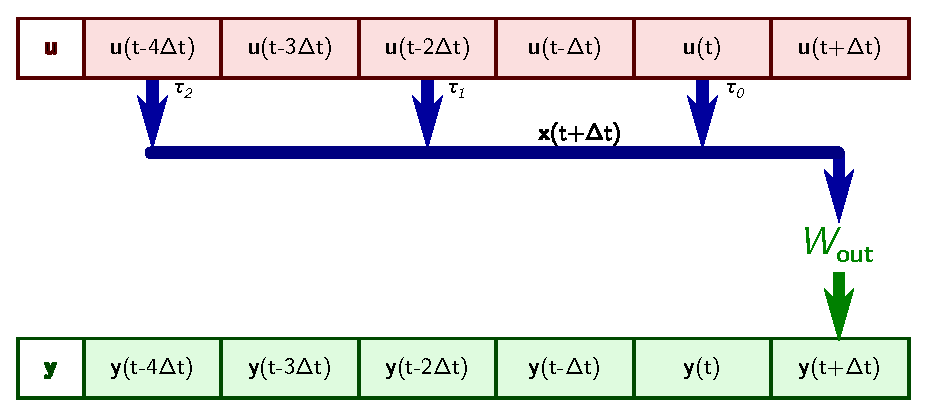
\includegraphics{figures/var-infer}
  \caption{Summary of the VAR method. Many time-delay taps $\tau_i$ of
    the signal $\bm{u}(t)$ (top, red) is collected into the tap vector
    $\bm{x}(t)$ (middle, blue). Here, there are three taps $\tau_1=0$,
    $\tau_2=2$, and $\tau_3=4$. These taps are then combined linearly
    by the output matrix $W_\text{out}$ to produce the next value of
    the VAR's output $\bm{y}(t)$ (bottom, green). To transform a whole
    time series input, this VAR process slides along the time axis
    from left to right.}
  \label{fig:var-infer}
\end{figure}

The output of the VAR is a linear transformation of this tap vector,
\begin{equation}
  \label{eq:var-y}
  \bm{y}(t + \Delta t) = W_\text{out}\;\bm{x}(t + \Delta t).
\end{equation}
This transformation process, from input to output, is summarized in
\cref{fig:var-infer}. Note the similarity to the RC method: the input
signal $\bm{u}(t)$ drives an internal state $\bm{x}(t)$ / $\bm{r}(t)$,
which is then linearly transformed into the output
$\bm{y}(t)$. However, the internal state $\bm{x}(t)$ of the VAR is
much simpler than that of most reservoirs, since it is constructed
directly from the input.

Once the taps $\tau_i$ are selected, the VAR can be trained in much
the same way as an RC. The VAR is fed an example input
$\bm{u}_\text{train}(t)$, which produces an example tap vector
$\bm{x}_\text{train}(t)$ via \cref{eq:var-x}. Finally, a $W_\text{out}$
that best maps this $\bm{x}_\text{train}(t)$ onto the example output
$\bm{y}_\text{train}(t)$ can be found via ridge regression, exactly as
in the RC case.

VARs can also be used for forecasting as well. Analogously to the RC
case, the VAR used for forecasting can be trained to reproduce the
example input as its output. Since the VAR output $\bm{y}(t + \Delta
t)$ depends only on $\bm{u}(t)$ at time $t$ and earlier, this amounts
to one step ahead prediction. Once trained, the VAR can do autonomous
prediction by replacing the input $\bm{u}(t)$ with the output
$\bm{y}(t)$ in \cref{eq:var-x}.

For practical reasons, in this thesis forecasting VARs have a modified
output equation
\begin{equation}
  \bm{y}(t + \Delta t) = \bm{u}(t) + W_\text{out}\;\bm{x}(t + \Delta t).
\end{equation}
This effectively changes the VAR from one step ahead prediction to
predicting the difference between the last value of the signal and the
next, in analogy to a discrete time integrator. Without this change,
the components of $W_\text{out}$ corresponding to $\bm{u}(t)$ would be
larger than the others. Since the ridge regression used to find
$W_\text{out}$ has a single regalurization parameter $\alpha$, it
works best when all components of $W_\text{out}$ have about the same
expected scale.

Once trained, either as a transformation or for prediction, a VAR can
be tested in the same ways as an RC.

Working with a VAR, by training it and using it, is very similar to
working with an RC. The most important difference is that using a VAR
completely sidesteps the issue of choosing an internal
reservoir. Building an ESN reservoir is a complicated process that
starts with the metaparameters listed in \cref{tab:esn-metaparameters}
and ends with a random realization of a network, usually of 100 nodes
or more. In contrast, building a VAR amounts to selecting which taps
$\tau_i$ to use, and how many.

However, the linear ESN solution in \cref{eq:esn-var-mat} is only
completely equivalent to a VAR with an infinite number of time delay
taps. VARs with a finite number of taps $k$ will approximate a VAR
with infitite taps under the right conditions as $k \rightarrow
\infty$\cite{bollt2021}, but if VARs are to be used as a replacement
for RCs, it is critical to know how good this approximation is in
practice. If an VAR requires thousands of taps to work, it may still
be simpler just to use an ESN.

Finally, these linear VARs suffer from the same drawbacks as the
linear ESN. Any practical replacement for an ESN would have to
reproduce the attractors of the systems they are trained on, as in
\cref{ch:low-connectivity}, and to do that, they need a non-linearity.

\section{Non-linear Vector Autoregressions (NVARs)}

% introduce nonlinearity in g, not f
% how does this fall out for quadratic g? (due to bollt)
% define NVAR(k), figure
% still simple, and as will be demonstrated, *can* reproduce attractors

\section{Practical Considerations}

% VAR/NVAR(k) approximates VAR/NVAR(inf), but how well? How many k do we need?
% NVAR proven for quadratic, but quadratic is insufficient (sym). what else?
% also, monomial features grow as O(k^n), which can get very bad. how little n?
% however, *if* all of that works out, NVAR dramatically fewer knobs than ESN

\section{Summary}

% summarize VAR, summarize NVAR, note possible problems addressed in next ch.
% note how *simple* it all is, in comparison
